\section{Zusammenwirken mehrerer Systeme}
\subsection{Regelkreis}
\begin{mdframed}[style=exercise,frametitle=Anforderungen:]
	\begin{itemize}[leftmargin=*]
		\item Stabilität: Regelkreis muss stabiles Verhalten zeigen (gilt
		      auch für instabile Systeme)
		\item Gutes Führungsverhalten: Die Differenz zw. Sollwert w(t) und
		      Istwert x(t) muss schnell klein werden.
		\item Gutes Störverhalten: Einfluss von Störgrößen soll vermindert
		      werden.
	\end{itemize}
\end{mdframed}

Grundstruktur des einschleifigen Regelkreises:

\includegraphics[width=0.9\columnwidth]{Figures/einschleifiger Regelkreis.png}

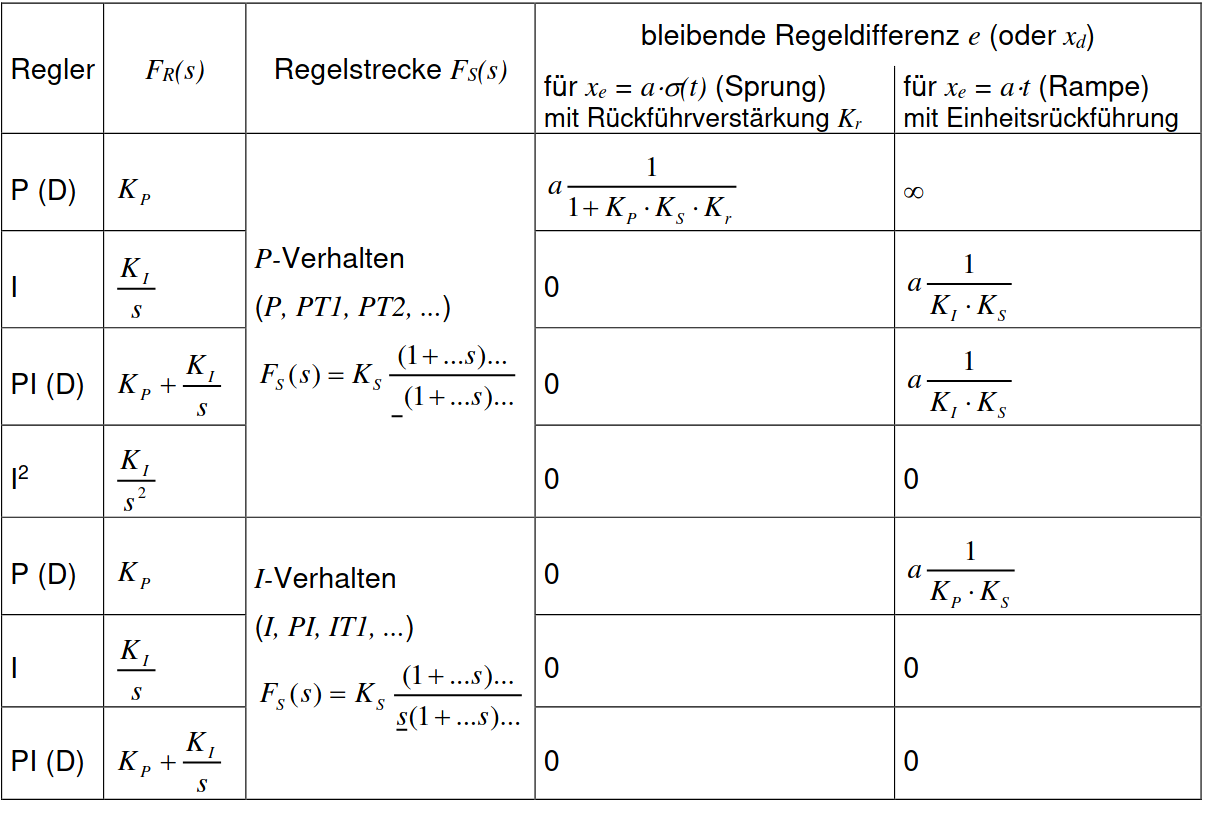
\includegraphics[width=0.98\columnwidth]{Figures/Reglerauswahl.png}


\subsection{Wurzelortskurven (WOK)-Verfahren}
\begin{mdframed}[style=exercise]
	Reglerfunktion $F_R$ in Reglerverstärkung und Reglerdynamik aufspalten:
	$F_R =K \cdot F_R ' $
\end{mdframed}

\includegraphics[width=0.94\columnwidth]{Figures/WOKkreis.png}
\[
	\Rightarrow F_w (s)= \dfrac {F_R \cdot F_S} {1+F_R \cdot F_S \cdot F_r}
\]

\begin{mdframed}[style=exercise]
	Dabei ist $F_o = F_R \cdot F_S \cdot F_r$ die Übertragungsfunktion des
	offenen Regelkreises. $F_o$ kann auch in faktorisierter Form angegeben
	werden:
\end{mdframed}

\begin{align*}
	F_w (s) & = F_R (s) \cdot F_S (s) \cdot F_r (s)
	\\ & =K \cdot F_R '(s) \cdot F_S (s) \cdot F_r (s)
	\\ & =K \cdot Q \cdot \frac{\prod_{u=1}^{m}\left(s-s_{\text {N}}\right)}{\prod_{v=1}^{n}\left(s-s_{\text {P }}\right)}
\end{align*}

Für eine Polstele, muss der Nenner von $F_w (s)$ Null werden:
\[
	\dfrac{F_R (s) \cdot F_S (s)}{1+F_o (s)} \Rightarrow 1+F_o (s) \stackrel{!}{=}0
\]

Daraus folgt:
\begin{align*}
	 & \Rightarrow 1+ K \cdot Q \cdot \frac{\prod_{M=1}^{m}\left(s-s_{\text {N }}\right)}{\prod_{v=1}^{n}\left(s-s_{\text {P }}\right)}         \\
	 & \Rightarrow \frac{\prod_{v=1}^{n}\left(s-s_{\text {P }}\right)}{\prod_{u=1}^{m}\left(s-s_{\text {N }}\right)} \stackrel{!}{=} -K \cdot Q
\end{align*}

K kritisch
\[ K_{krit} = |K| \cdot \dfrac{\prod |s_{P}|}{\prod |s_{N}|}\]

\subsection{Konstruktion der WOK}

\[ ax^2+bx+c \qquad z_{1,2} = \dfrac{-b \pm \sqrt{b^2 -4ac}}{2a}\]

\begin{mdframed}[style=exercise]
	\begin{enumerate}[leftmargin=*]
		\item Alle n Äste beginnen in den n POLEN $s_pov$
		\item m Äste der WOK enden für K $\rightarrow \pm \infty$
		\item n -m Äste der WOK enden für K $\rightarrow \pm \infty$ im Unendlichen
		\item Die n-m ins Unendliche strebende Äste der WOK haben Asymptoten,die\\
		      a) im Wurzelschwerpunkt
		      \[S_{w}=\frac{\sum_{v=1}^{n} s_{P}-\sum_{u=1}^{m} s_{_{N}}}{n-m} 
                        = \dfrac{\textnormal{Polst.}- \textnormal{Nullst.}}{\textnormal{Polst. Überschuss}}\]
		      b) mit der reellen Achse die Winkel\\
			  Polst. Überschuss 1 $\Rightarrow 180^{\circ}$, 2 $\Rightarrow 90/270^{\circ}$\\
		      $\varphi_{k}=\frac{(2 k-1) \cdot 180^{\circ}}{n-m}$ für KQ > 0\\
		      k = 1,2,3,\dots,n-m
		\item Die Punkte liegen auf der reellen Achse, oder symmetrisch zur reellen Achse
		\item Ein Punkt s auf der reellen Achse ist dann ein Punkt der WOK, wenn sich bei KQ > 0 (KQ<0)
		      rechts von ihm eine ungerade (gerade) Anzahl von Polen $s_{P}$ und (+) Nullstellen $s_{N}$ befindet.
	\end{enumerate}

	Achtung: WOK nicht anwendbar, wenn Übertragungsfunktionen nicht rationale (z.B. Regelkreis mit Totzeitverhalten!)
\end{mdframed}

\subsection{Nyquist Kriterium}
\begin{center}
	\includegraphics[width=.45\textwidth]{Figures/Nyquist.png}
\end{center}
Frequenzgangfunktion des offenen Regelkreises:
\[
	F_o (j\omega) = F_r (j\omega) \cdot F_R (j\omega) \cdot F_S (j\omega)
\]

Ausgangssignal:
\begin{align*}
	x_a(t) & =-F_r (j\omega) \cdot F_R (j\omega) \cdot F_S (j\omega) \cdot
	x_{e0}sin(\omega t)                                                    \\
	       & = -F_0 (j\omega) \cdot x_e (t)
\end{align*}

Regler und seine Parameter werden so gewählt,\\ dass $\omega = \omega_{krit}$ gilt:
\[
	-F_0 (j\omega_{krit})=1 \text{ oder } F_0 (j\omega_{krit})=-1 \texttt{ (Schwingbedingung)}
\]

\begin{mdframed}[style=exercise]
	Die Schwingbedingung ist erfüllt, wenn die Ortskurve von $F_1 (j\omega)$
	durch den kritischen Punkt ($P_{krit} = -2+j0$) der komplexen $F_0$-Ebene
	geht.

	An diesem Punkt kann man $\omega_{krit}$ ablesen (damit kann der Regelkreis
	Dauerschwingungen ausführen).

	Für größere $\omega$ ist das System instabil, für kleinere stabil.
\end{mdframed}

\includegraphics[width=0.94\columnwidth]{Figures/Nyquistwkrit.png}

\begin{mdframed}[style=exercise]
	Falls F(s) des offenen Kreises keine Pole in der rechten Halbebene hat und
	nur max. 2 im Ursprung der s-Ebene, ist der Regelkreis stabil, wenn der
	kritische Punkt von $\omega$ immer links von s = -1 + 0j liegt.

	\footnotesize
	(gilt immer wenn der offene Kreis stabil ist)
\end{mdframed}

Zur Auswertung des Nyquist-Kriteriums im Bode Diagramm, spaltet man die Ortskurve nach Betrag
A = |$F_0 (jw)$ und Phase $\varphi$ = $F_0(jw)$

\includegraphics[width=0.94\columnwidth]{Figures/Nyquist_Bode.png}

Falls die Bedingung nicht funktioniert, wird die allgemeine Formulierung verwendet:

\includegraphics[width=0.94\columnwidth]{Figures/Allgemein_Nyquist.png}

\begin{mdframed}[style=exercise]
	Der geschlossene Regelkreis ist stabil, wenn der Fahrstrahl von $P_{krit}$ = -1 +j0
	zu $F_0 (jw)$ für wachsendes $\omega$ von +0 bis +$\infty$ eine Winkeländerung
	$^{\omega=+\infty}_{\omega=+0} \Delta \phi _{soll} = n_r \cdot$ 180° $+n_a \cdot$ 90°
	erfährt.\\
	$n_r$: Anzahl der Pole rechts der imaginären Achse\\
	$n_a$: Anzahl der Pole auf der imaginären Achse
\end{mdframed}

\subsubsection{Phasenrad/Phasenreserve:}

\begin{itemize}[leftmargin=*]
	\item[] Aus Bodediagramm ablesen: Bei Verstärkung von 1
	\item[] Winkeln von -180° nach oben rechnen
	\item befriedigendes Verhalten bei Störungen gilt: $\varphi _R \geq 30\circ$
	\item gutes Verhalten (überschwingungsarm) gilt: $\varphi _R \approx  60\circ$
	\item gutes Verhalten (überschwingungsfrei) gilt: $\varphi _R \geq 80^\circ$
\end{itemize}

\subsection{Einstellregler Ziegler/Nichols}
{\centering
\includegraphics[width=0.9\columnwidth]{Figures/ZieglerNich.png}}

\subsubsection{Betragsoptimum}
bei einer dominierenden  Zeitkonstante ($T_d$) in der Regelstrecke
\[
	F_{PI} = K_R \left(1 + \dfrac{1}{T_d \cdot s}\right) \qquad K_R =\dfrac{T_d}{2 \cdot K_{Strecke} \cdot T_{\sum}}
\]

\subsubsection{Symmetrisches Optimum}
mehreren Zeitkonstanten (nur reelle Pole)
\[
	F_{PI} = K_R \left(1 + \dfrac{1}{4T_{\sum} \cdot s}\right) \qquad K_R =\dfrac{1}{2 \cdot K_{Strecke} \cdot T_{\sum}}
\]

\raggedright
\begin{mdframed}[style=exercise, frametitle=Störgrößenaufschaltung:]
	Falls Angriffsort einer Störgröße bekannt,kann man wie im Bild kompensieren.
	Vorteil: einfacher Regler Entwurf, deutlich schnellere Ausregelung.
\end{mdframed}

\includegraphics[width=0.9\columnwidth]{Figures/Stoergoesenschaltung.png}


\begin{mdframed}[style=exercise, frametitle=Vorsteuerung:]
	Geeignet, falls kein Kompromiss für gutes Stör und Folgeverhalten.
	Regler ist auf gutes Störverhalten ausgelegt. Mit $F_{Rv}$ wird ein schnelles Folgen
	auf Führungssignale w(t) erreicht.
\end{mdframed}

\includegraphics[width=0.9\columnwidth]{Figures/Vorsteuerung.png}


\begin{mdframed}[style=exercise, frametitle=Kaskadenregelung:]
	Ineinander geschachtelte Regelkreise (innere Regelkreise „schneller“). „Innere“
	Störungen können bereits innen ausgeregelt werden. Können von Innen nach Außen in Betrieb genommen werden.
\end{mdframed}

\includegraphics[width=0.9\columnwidth]{Figures/Kaskadenregelung.png}

\newpage